\chapter{Mathematical introduction}
\label{chap:mathIntro}
The modern approach to the closed system dynamics is using \emph{differential geometry} formalism. Before we get to the quantum mechanics itself, let's introduce this formalism and recapitulate some definitions of this branch of mathematics. More detailed notes can be found for example in \cite{lu}, or \cite{fecko}. Because sometimes in physical theory the mathematical background is blurred, the basics of differential geometry will be recapitulated here. This chapter should lead the reader to better understanding of the physical theory in following chapters, but is not essential for performing the analysis of driving in Hamiltonian systems, which is the main goal of the thesis.

Let's have a manifold $\M$ over the field of complex numbers $\mathbb C$, usually complex numbers. Curves on this manifold are parametrized by some real interval:
$$\gamma:\R \supset (P_i,P_f) \rightarrow \M\; \qquad \xi\mapsto \gamma(\xi) \text{  for } \xi \in (P_i,P_f) .$$ 
The space of functions is $\FM\equiv\{f:\M\rightarrow \C\}$.


To define \bluee{\emph{vectors}} on $\M$, we need to make sense of the \emph{direction}. It is defined using curves satisfying 
$$\gamma_1(0)=\gamma_2(0)\equiv P$$
$$\der{}{t}x^i(\gamma_1(t))\big|_{t=0}=\der{}{t}x^i(\gamma_2(t))\big|_{t=0}.$$
Taking the equivalence class created by these two rules, sometimes noted as $\bluee{[\gamma]}=\bluee v$, we have an element of the tangent space to $\M$. We will use standard notation for the \bluee{tangent space of $\M$} in some point $P\in\M$ as $\bluee{\T_P\M}$. Cotangent space is denoted as $\blueee{\T^*_P\M}$. Unifying all \bluee{tangent}, resp cotangent spaces over all $x$ we get tangent and cotangent bundle, \bluee{$\TT\M$} and $\TT^*\M$ respective. To generalize this notation to higher tensors, we denote $\T_P\M\in \TT^1\M$, $\T^*_P\M\in \TT_1\M$. This gives us the possibility to increase the order, leading to $p-$times \bluee{contravariant} and $q-$times \blueee{covariant} tensors. These are usually denoted $\TT^{\bluee p}_{\blueee q} \M$. Tensor space in point $P\in\M$ is denoted ${\TT_P}^{\bluee p}_{\blueee q} \M$
Using the congruence of curves on $\M$, the expression 
\begin{equation}
    \bluee{\der{}{\xi}}f\circ \gamma(\xi)\bluee{\Big|_{\xi=0}}
\end{equation}
has a good meaning, and we can define the \emph{vector} in some $P\in\M$ as
\begin{equation}
    \bluee{\bm v}: \FM\rightarrow \mathbb F \qquad f\mapsto \bluee{\bm v[}f\bluee ]\equiv \frac{\bluee \d f(\gamma(\xi))}{\bluee{\d \xi}}\bluee{\Big|_P} \equiv \bluee{\partial_\xi\Big|_P} f .
\end{equation}
It holds that $\bluee{\bm v}\in \bluee{\T_P\M}$ and can be expressed as the \emph{derivative in direction},\footnote{
        The direction itself is usually denoted as
        \begin{equation}
            \frac{\D}{\d\bm\alpha}\gamma(\xi),
        \end{equation}
        where the "big D" notation is used to point out that it's not a classical derivative, but it maps curves to some entirely new space of directions.
    } 
which can be understood in coordinates as
\begin{equation}
    \bluee{\bm v[}f\bluee ] = \bluee{\der{}{\bm v}} f\circ \gamma(\xi)\bluee{\Big|_{\xi=0}}=v^\mu\bluee{\der{}{x^\mu}} f(\bm x)\Big|_{P}.
\end{equation}
The directional derivative will be denoted $\bm\nabla_v$
and in basis $\bluee{\bm e_i} \equiv \bluee{\partial/\partial x^i}$ it becomes
$$\bm\nabla=\bluee(\bluee{\bm e_1}, \bluee{\bm e_2},\bluee{\bm e_3}).$$


During the whole thesis, the \emph{abstract indices} (written by Greek letters) and \emph{pointer indices} (written using Latin letters) will be differentiated. Abstract indices show the rank of the tensor, meaning \emph{how many empty slots for contraction the tensor has}. Pointer indices extract specific number from the tensor. For example
$$t^\mu_{\nu\kappa} \in \TT^1_2\M, \quad \text{ whilst for some }i,j,k\in\N: t^i_{jk}\in \mathbb C.$$

For \emph{Tensor contraction}, the index notation will be used. When it is clear what type of tensors we are operating with, the object notation can be used, for example $t(\bluee{\bm u},\bluee{\bm v})\equiv t_{\mu\nu}\bluee{\bm u^\mu \bm v^\nu}$. The contraction can also be noted using contraction operator $\mathbf C$, when it is clear which indices are contracted, or when it does not matter which of them are.

Now we have the notation to define one strong structure on manifolds -- \emph{metric tensor}. 
\begin{definition}[Metric tensor]
If the 2-form $g_{\mu\nu}\in\TT^0_2\M$ is
\begin{itemize}
    \item linear in second argument: $\forall \alpha,\beta\in\C;\; \bluee{\bm u,\bm v,\bm w}\in \bluee{\TT^1\M}: \; g(\bluee{\bm u},\alpha\bluee{\bm v}+\beta \bluee{\bm w}) = \alpha g(\bluee{\bm u},\bluee{\bm v})+\beta g(\bluee{\bm u},\bluee{\bm w})$,
    \item hermitian: $\forall \bluee{\bm v,\bm w}\in \bluee{\TT^1\M}: \; g(\bluee{\bm v},\bluee{\bm w})=g(\bluee{\bm w},\bluee{\bm v})^*$,
    \item non-degenerate: $\forall \bluee{\bm v}\in\bluee{\TT^1\M}$ the function $\bluee{\bm w}\mapsto g(\bluee{\bm v},\bluee{\bm w})$ is not identically zero,
\end{itemize} 
we call $g_{\mu\nu}$ a \emph{metric tensor}. The $^*$ marks complex conjugation.
\end{definition}

We will often require \emph{differentiable metric tensor}, or at least almost everywhere differentiable\footnote{Almost everywhere means \emph{with an exception to the submanifold of zero measure}. Often it means only a few point singularities.}. That will assure that \emph{covariant derivatives} and \emph{parallel transport} are well-defined almost everywhere. 




Vectors of tangent space to some manifold can be compared only within one such space. To perform some tensor operations we need to transport them to some common tangent space. This can be done using the \emph{parallel transport} which is connected to the notion of \emph{covariant derivative}.

\begin{definition}[Covariant derivative]
\label{def:covariantDerivative}
    $\bm\nabla_{\bluee{\bm v}}$ is called the covariant derivative in a direction $\bluee{\bm v} \in \bluee{\T_P\M}$, if $\forall f\in\FM, \; \bm A,\bm B\in \TT^{\bluee p}_{\blueee q} \M,\; \alpha\in\C: $
    \begin{itemize}
        \item $\bm\nabla_{\bluee{\bm v}}:\; \TT^{\bluee p}_{\blueee q} \M \rightarrow {\TT_P}^{\bluee p}_{\blueee q} \M$
        \item $\bm\nabla_{f\bluee{\bm v}}\bm A=f\bm\nabla_{\bluee{\bm v}} $ (ultralocality in a direction)
        \item $\bm\nabla_{\bluee{\bm v}}(\bm A+\alpha \bm B)=\bm\nabla_{\bluee{\bm v}}\bm A+\alpha\bm\nabla_{\bluee{\bm v}}\bm B$ (linearity in argument)
        \item $\bm\nabla_{\bluee{\bm v}}(\bm{AB})=(\bm\nabla_{\bluee{\bm v}}\bm A)\bm B+\bm A(\bm\nabla_{\bluee{\bm v}}\bm B)$ (Leibniz rule)
        \item $\bm\nabla_{\bluee{\bm v}}(\mathbf C \bm A)=\mathbf C \bm\nabla_{\bluee{\bm v}}(\bm A)$ (commutation with contraction)
        \item $\bm\nabla_{\bluee{\bm v}}f=\bluee{\bm v[}f\bluee ]\equiv\bluee{\bm v^\beta \bm \d_\beta} f$ (operation on functions)
    \end{itemize}
\end{definition}

% \begin{definition}[Coavariant differential]
%     For $\bluee{\bm v} \in \bluee{\T_P\M}, \bm A\in \TT^{\bluee p}_{\blueee q} \M$, the covariant differential is defined as
%     $$\bm\nabla:\; \TT^{\bluee p}_{\blueee q} \M \rightarrow {\TT_P}^{\bluee p}_{\blueee{q+1}} \M
%     \text{, for which } \bm\nabla_{\bluee{\bm v}}\bm A^{\alpha\dots}_{\beta\dots}=\bluee{\bm v^\gamma} \bm\nabla_{\gamma}\bm A^{\alpha\dots}_{\beta\dots}$$
% \end{definition}

% \begin{definition}[Pseudoderivative]
%     \label{def:pseudoderivative}
%         $\bm P$ is called a pseudoderivative of type $p,q$, if $\forall f\in\FM, \; \bm A,\bm B\in \TT^{\bluee p}_{\blueee q} \M: $
%         \begin{itemize}
%             \item $\bm P:\; \TT^{\bluee p}_{\blueee q}\M\rightarrow \TT^{\bluee p+m}_{\blueee q+n}\M$
%             \item $\bm P f=0$ (ultralocality)
%             \item $\bm P(f\bm A+\bm B)=f\bm P\bm A+\bm P \bm B$ (linearity)
%             \item $\bm P(\bm{AB})=(\bm{PA})\bm B+ \bm A(\bm{PB})$ (Leibniz rule)
%             \item $\bm M \mathcal C \bm A=\mathcal C\bm{MA}$ (commutation with contraction)
%         \end{itemize}
% \end{definition}
    
\begin{definition}[Parallel transport]
    Parallel transport of tensors in tensor field $A\in \TT^{\bluee p}_{\blueee q} \M$ along some path $\gamma$ going from $P_i\in\M$ to $P_f\in\M$ is denoted
    \begin{align*}
        \Par_\gamma:\; {\TT _{P_i}}^{\bluee p}_{\blueee q}\M&\rightarrow {\TT_{P_f}}^{\bluee p}_{\blueee q}\M\\
        A|_{P_i} &\mapsto \Par_\gamma \bm A|_{P_f}.
    \end{align*}
\end{definition}
This means that the parallel transport takes a tensor at some ${\TT_{P_i}}^{\bluee p}_{\blueee q} \M$ and transports it to ${\TT_{P_f}}^{\bluee p}_{\blueee q} \M$.  Those two tensors belong to the same tensor field, but are essentially different. One cannot simply add or subtract them. For that they need to be transported into the same tensor space $\TT^{\bluee p}_{\blueee q} \M$ using the parallel transport.

% \begin{definition}[Coordinate derivative]
%     Associate the derivative $\bm \partial$ with coordinates $x^\mu$ on some $O\subset\M$ as
%     $$\bm \partial (\bm \d x^j)=0.$$
% \end{definition}
% Then the coordinate derivative of any tensor can be expressed as
% \begin{equation}
%     \bm \partial_\rho \bm A^{\alpha,\dots}_{\beta\dots} = \bm A^{a,\dots}_{b\dots,q}\bm \d_\alpha x^q \bm \d_\alpha x^b  \dots \frac{\bm \partial^\beta}{\bm \partial x^a},
% \end{equation}
% where on the expression on the left means \emph{taking the covariant derivative of the tensor} and the expression on the right \emph{multiplying the basis of the tensor space by derivative of the elements of tensor $\bm A$}.
% \begin{thm}[Difference of covariant derivatives]
%      Difference of two covariant derivatives, i.e. two objects $\bm \nabla$, $\bm{\tilde\nabla}$ satisfying Def. \ref{def:covariantDerivative},
%       $$\bm\nabla-\bm{\tilde\nabla}$$
%     is a pseudoderivative from Def. \ref{def:pseudoderivative}.
% \end{thm}

Another object, which will be heavily used further on is the \emph{affine connection}. It is generally defined as the difference of covariant and coordinate derivative
$\bm \Gamma\coloneqq \bm\nabla-\bm\partial$. Because this definition is rather complicated and requires some additional theory, only the \emph{connection on metric spaces} will be provided here. 

\begin{definition}[Connection and Christoffel symbols]
The Affine connection on metric spaces can be defined as
    \begin{equation}
        \Gamma^{\alpha}_{\mu\nu} \coloneqq \frac{1}{2}g^{\alpha \beta}\left(g_{\beta\mu,\nu}+g_{\nu\beta,\mu}-g_{\mu\nu,\beta}\right),
    \end{equation}
    where we used comma notation for the coordinate derivative. Its elements are called the \emph{Christoffel symbols}.
\end{definition}
    The covariant derivative of a vector $\bluee{\bm a}\in \T_P\M$ for manifold with coordinates $x^\mu$ can be expressed as (using $D$ notation instead of $\bm \nabla$)
    \begin{equation}
        \Der{\bluee{\bm a^\mu}}{x^\nu}=\bluee{\bm a_{\;,\nu}^\mu}-\Gamma^\mu_{\alpha\beta} x^\alpha \bluee{\bm a^\beta}
    \end{equation}
    and for $\blueee{\bm\alpha\in} \T_P^*\M$ it is
\begin{equation}
    \Der{\blueee{\bm \alpha_\mu}}{x^\nu}=\blueee{\bm \alpha_{\mu,\nu}}-\Gamma^\alpha_{\mu\beta}x^\beta \blueee{\bm \alpha_\alpha}
\end{equation}

The vector $\bluee{\bm v}\in \T_P\M$ is said to be parallel transported along curve $\gamma(\lambda)$, if its covariant derivative vanishes along $\gamma(\xi)$
\begin{equation}
    \Der{\bluee{\bm v^\mu}}{\xi}=0.
\end{equation}

\section{Fiber bundle}
\label{sec:bundleDef}
Sometimes one needs to add additional structure to every point on manifold. These structures are usually imagined like fibers going from the manifold, similarly to the hair going from your head.

At every point of the manifold we introduced a tensor space. This structure can be described by so-called \emph{fiber bundles}. From classical mechanics one might recognize the space of all vectors, \emph{vector bundle}, as a union of all vectors from the phase space $\cup_x\T_x\M$.
\begin{definition}[Fiber bundle]
    \label{def:fiberBundle}
    Structure 
\begin{center}
    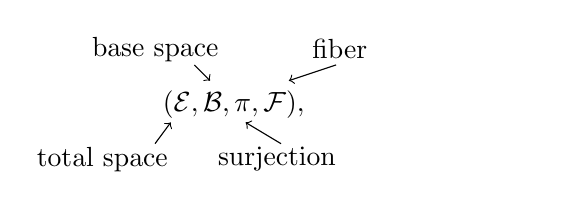
\begin{tikzpicture}[remember picture]
        \node {\(\displaystyle(
            \mathcal{E},\mathcal{B},\pi,\mathcal{F}),
            \)};
            \node[text width=3cm] at (-1,-0.7) {total space};
            \node[text width=3cm] at (1.3,-0.7) {surjection};
            \node[text width=3cm] at (-0.3,0.7) {base space};
            \node[text width=3cm] at (2.5,0.7) {fiber};
            \draw[->] (-1,-0.5)--(-0.8,-0.23);
            \draw[->] (-0.5,0.5)--(-0.3,0.30);
            \draw[->] (0.6,-0.5)--(0.15,-0.23);
            \draw[->] (1.3,0.5)--(0.7,0.3);
        \end{tikzpicture}
\end{center}
    for topological spaces $\mathcal{E}$, $\mathcal{B}$, $\mathcal F$ and continuous surjection $\pi: \mathcal{E}\rightarrow \mathcal{B}$ satisfying a local triviality, is called a \emph{Fiber bundle}. The local triviality means that $\mathcal{B}$ is connected\footnote{Connected mean, it can't be represented as a union of two and more disjoint sets} and for every $x\in \mathcal{B}$, there is an open neighborhood $\mathcal{U}\subset \mathcal{B}$ \emph{(trivializing neighborhood)} such that there exists a homeomorphism from $\mathcal{U}$ to so-called \emph{product space}
    $$\phi: \pi^{-1}(\mathcal{U})\rightarrow \mathcal{U}\times \mathcal{F},$$
    such that $\pi^{-1}\circ \pi(\mathcal{U})=\mathcal{U}$. Plus there exist natural projection from $\mathcal{U}\times \mathcal{F}$ to $\mathcal U$, setting the coordinate in fibers to zero. The structure can be visualized as follows: 
    % See the mappings on Fig. \ref{fig:bundle}.

    \begin{figure}[H]
        \centering
        \begin{tikzpicture}[->,>=stealth',auto,node distance=3.0 cm,
            thick,main node/.style={}]
            
            \node[main node] (1) {$\pi^{-1}(\mathcal U)$};
            \node[main node] (2) [right of=1] {$\mathcal U$};
            \node[main node] (3) [right of=2] {$\mathcal U\times \mathcal F$};
            
            \path[every node/.style={}]
            (1) edge node [above] {$\pi$} (2)
            (3) edge node [above] {projection} (2)
            (1) edge[bend right] node [below] {$\phi$} (3);
        \end{tikzpicture}
    \end{figure}

\end{definition}
Because the projections of products are open maps, $\pi: \mathcal{E}\rightarrow \mathcal{B}$ must be an open map. The manifolds at every point $x\in \mathcal{F}$ are all locally diffeomorphic to each other.

With the analogy to the hair on your head, one can say that $\mathcal B$ is the head, $\mathcal F$ is the hair, $\pi$ applied on the hair returns the point on your head and $\mathcal E$ is the head with all the hairs.


% \section{\red{Vector Bundle}}
% Conversely, given a fiber bundle (E, X, $\pi$, Rk) with a GL(k) cocycle acting in the standard way on the fiber Rk, there is associated a vector bundle. This is sometimes taken as the definition of a vector bundle


% \subsection{Connection on vector bundles}
% \citep{lu}[chap. 10.1]
% Connection maps vector from tangent space to base manifold $\mathcal{X}$ with some element from total space $\mathcal{E}$ to total space
% $$\Gamma: \mathcal{X}\times \mathcal{E}\rightarrow \mathcal{E}$$
% such, that
% \begin{itemize}
%     \item $\Gamma_X s$ is $\mathcal{F}-$linear in $X$ and $\R-$linear in $s$
%     \item Leibniz rule for $f\in \mathcal{C}^\infty$ is satisfied: $\Gamma_X(f s) = (X f)s+f\Gamma_X s$
% \end{itemize}


% \subsection{Metric on vector bundles}
% Map
% $$g_{\mu\nu}: \mathcal{B}\times \mathcal{B} \rightarrow \R$$

% \section{\red{Sections}}
% \label{sec:section}
% \emph{Section} is a function
% $$f:\mathcal{B}\rightarrow \mathcal{F},$$
% such that $\pi(f(x))=x$ for $\forall x\in \mathcal{B}$. This defines new manifold cutting throw $\mathcal{E}$.

% \textcolor{red}{Sectioning of fiber bundles creates vector spaces}


% \section{Pull-back and push forward}
% Push-forward and pull-back are used to transport vectors and covectors between manifolds. Let's have two manifolds $\M$, $\mathcal{N}$, a smooth mapping $\phi$ and functions $f,\tilde f$ such that
% \begin{align*}
%     \phi&:\M\rightarrow \mathcal{N}\qquad x\mapsto \phi x\\
%     \tilde f&:\mathcal{N}\rightarrow \R 
% \end{align*}
% \emph{Pull-back of the function} then defines a new function $
% f:\M\rightarrow \R $ as
% $$\phi^*:\F \mathcal{N}\rightarrow \F\M \qquad  \tilde f\mapsto f=(\phi^*\tilde f)(x)\equiv \phi^*\tilde f(x) =\tilde f(\phi x).$$
% \emph{Push-forward of a vector} is defined as
% $$\phi_*: \T_x\M \rightarrow \T_{\phi x}\mathcal N\qquad \phi_* 
% \Der{\gamma(\xi)}{\xi}\Big|_x=\Der{\phi \gamma(\xi)}{\xi}\Big|_x$$
% and \emph{pull-back of a covector} $\bm\tilde\alpha\in \T_{\phi x}\mathcal N$ is
% $$\phi^*: \T_{\phi x}\mathcal N\rightarrow \T_x\M  \qquad (\phi^*\bm \tilde\alpha)_\mu v^\mu\big|_x= \tilde\alpha_\mu (\phi_* \bm v)^\mu\big|_{\phi x}.$$
% If $\phi$ has a smooth inversion, i.e. it is a dippheomorphism, we can define pull-back of vectors as
% \begin{equation}
%     \phi^*=\phi_*^{-1}
% \end{equation}
% and push-forward of covectors
% \begin{equation}
%     \phi_*=(\phi^{-1})^*
% \end{equation}




% \section{\red{Parallel transport on vector bundles}}
% \textcolor{blue}{this is what we need}
% Parallel transport of vector $V$ along curve $\gamma$ will be denoted
% $$\Par_\gamma V.$$



% \section{\red{Antisymmetric tensors}}
% $p-$form $\bm A\in \TT_p \M$ is called \emph{antisymmetric}, if changing the order of the indices has impact only on the sign, symbolically
% $$A_{i_1\dots i_p} = \sign(\sigma)A_{i_{\sigma_1}\dots i_{\sigma_p}},$$
% where $\sigma$ is some permutation.\emph{Antisymmetrisation} is defined as a normalized sum over all permutation
% \begin{equation}
%     A^{[i_1\dots i_p]}\equiv \frac{1}{p!}\sum_\sigma A^{[i_{\sigma_1}\dots i_{\sigma_p}]}. 
% \end{equation}

% The \emph{wedge product} of $A\in \TT_p \M$ and $B\in \TT_q \M$ is antisymmetrisation of the tensor product in the sense
% \begin{equation}
%     A\wedge B\equiv \frac{(p+q)!}{p!q!} A^{[i_1\dots i_p}\otimes B^{i_1\dots i_q]}
% \end{equation}

\section{Riemannian geometry}
Let's briefly mention some definitions and theorems from Riemannian geometry, which will be used later on.
\begin{definition}[Riemannian manifold]
    Manifold is called Riemannian, iff it's equipped with positive definite metric tensor.
\end{definition}
\begin{definition}[Connected manifold]
    Manifold is connected, iff the distance between two points is infimum of the lengths of curves joining the two points.
\end{definition}
\begin{definition}[Compact manifold]
    Manifold is said to be compact if its every open cover has a finite subcover.
\end{definition}
\begin{definition}[Geodesical completeness]
    A manifold is said to be geodesically complete if its every geodesic can be extended to infinite values of their affine parameter. 
\end{definition}
This condition holds if the space does not contain any singularities. It is a coordinate-independent notion.
\begin{definition}[Geodesic maximality]
    A manifold is said to be geodesically maximal if it is either geodesically complete, or every non-complete geodesic (such that cannot be extended to infinite values of their affine parameter) ends in a singularity.
\end{definition}
Geodesic maximality is coordinate dependent notion, only if the manifold is geodesicaly complete.


\begin{thm}[Von Neumann-Wigner]\citep{landau}[page 305]
    \label{thm:n-2}

    This, sometimes called the Non-Crossing Theorem, states that the eigenvalues of Hermitian matrix driven by $N$ continuous real parameters forms at maximum $(N-2)$-dimensional submanifold.
\end{thm}


\begin{thm}[Hopf-Rinow Theorem]\citep{petersen}[p.125]
    \label{thm:hopf-Rinow}


    For connected Riemannian manifold $\M$ with the metric $g$, following are equivalent:
    \begin{itemize}
        \item $(\M,g)$ is geodesically complete, i.e. all geodesics are infinite
        \item $(\M,g)$ is geodesically complete at some point $P$, i.e. geodesics going through $P$ are infinite
        \item $(\M,g)$ satisfies the Heine-Borel property, i.e. every closed bounded set is compact
        \item $(\M,g)$ is complete as a metric space.
    \end{itemize}
\end{thm}
\begin{thm}[Modified Hopf-Rinow Theorem]\citep{claudio}[Chapter 3]
    \label{thm:hopf-Rinow_modified}

    For connected Riemannian manifold $\M$ with the metric $g$, any two points on $\M$ can be joined with a minimizing geodesic.
\end{thm}
This generally means that in a space with singularity exists such points, which cannot be connected with the rest of the manifold using geodesics. In General relativity, this area is for example below the event horizon of black holes.

\begin{thm}\citep{claudio}[Chapter 3]
    \label{thm:compact}

    A compact Riemannian manifold is geodesically complete.
\end{thm}





\section{Geometry in 2 dimensions}
An important tensor in differential geometry is the \emph{Riemann tensor}
\begin{equation}
    R^\alpha_{\;\;\beta\gamma\delta}\coloneqq \Gamma^\alpha_{\;\;\beta\delta,\gamma}-\Gamma^\alpha_{\;\;\beta\gamma,\delta}+\Gamma^\mu_{\;\;\beta\delta}\Gamma^\alpha_{\;\;\mu\gamma}-\Gamma^\mu_{\;\;\beta\gamma}\Gamma^\alpha_{\;\;\mu\delta}.
\end{equation}
\emph{Ricci tensor} can be defined as its contraction 
\begin{equation}
    R_{\alpha\gamma}\coloneqq R^\mu_{\;\;\alpha\mu\gamma},
\end{equation}
which is second order symmetric tensor.
\emph{Ricci scalar}, describing the curvature on manifold, is defined as contraction of the Ricci tensor
\begin{equation}
    R\coloneqq R^\mu_{\;\;\mu}.
\end{equation}
This can be simplified for 2-dimensional manifold as
\begin{equation}
    R=\frac{2}{g_{22}}\left(\Gamma^1_{\;22,1}-\Gamma^1_{\;12,2}+\Gamma^1_{\;11}\Gamma^1_{\;22}+\Gamma^1_{\;12}\Gamma^2_{\;22}-\Gamma^1_{\;21}\Gamma^1_{\;12}-\Gamma^1_{\;22}\Gamma^2_{\;12}\right).
    \label{eq:Ricci2D}
\end{equation}
Another possibility to express the Ricci tensor, see \citet[eq. 6,7]{geometricTensorLipkin}, is
\begin{equation}
    R=\frac{1}{\sqrt{\abs{g}}}(\mathcal{A}+\mathcal{B}),
\end{equation}
for
\begin{align}
    \mathcal{A}&\coloneqq \left(\frac{g_{12}}{g_{11}\sqrt{\abs{g}}}g_{11,2}-\frac{1}{\sqrt{\abs{g}}}g_{22,1}\right)_{,1}\\
    \mathcal{B}&\coloneqq \left(\frac{2}{\sqrt{\abs{g}}}g_{12,1}-\frac{1}{\sqrt{\abs{g}}}g_{11,2}-\frac{g_{12}}{g_{11}\sqrt{\abs{g}}}g_{11,1}\right)_{,2}.
\end{align}
This equation turned out to be less numerically stable, therefore Eq. \ref{eq:Ricci2D} will be user later on for calculating the Ricci tensor.

